\documentclass[conference]{IEEEtran}

\usepackage{cite}
\usepackage{amsmath,amssymb}
\usepackage{graphicx}
\usepackage{booktabs}
\usepackage{array}
\usepackage{url}
\usepackage{balance}

% Overleaf/local image search paths
\graphicspath{{./}{eda/plots/}{figures/}}

\title{Regime-Adaptive Multimodal Transformer for Cross-Market Equity Forecasting\\
\large HMM Regime Detection, Feature Engineering, and XGBoost Baseline}

\author{
\IEEEauthorblockN{1\textsuperscript{st} Vivek Vishnoi (Roll: 230119)}
\IEEEauthorblockA{\textit{B.Tech CSAI} \\
\textit{Rishihood University}\\
Sonipat, India \\
vivek.23csai@nst.rishihood.edu.in}
\and
\IEEEauthorblockN{2\textsuperscript{nd} Shivansh Gupta (Roll: 230054)}
\IEEEauthorblockA{\textit{B.Tech CSAI} \\
\textit{Rishihood University}\\
Sonipat, India \\
shivansh.g23@nst.rishihood.edu.in}
}

\begin{document}
\maketitle

\begin{abstract}
This report presents Phase-1 deliverables for cross-market equity forecasting using one U.S. stock (JPM) and four Indian stocks (RELIANCE, TCS, HDFCBANK, EPIGRAL). The current phase focuses on exploratory diagnostics, hidden Markov model (HMM) regime detection, a 36-column engineered feature table, and a walk-forward XGBoost baseline. The objective is to establish technically reliable foundations before introducing heavier deep architectures. We enforce temporal causality using T-1 time-zone alignment for cross-market linkage features to avoid look-ahead bias. Results show moderate directional performance with ticker-dependent risk-adjusted outcomes, motivating multimodal extension in later phases.
\end{abstract}

\begin{IEEEkeywords}
equity forecasting, hidden Markov model, regime detection, feature engineering, XGBoost, cross-market learning
\end{IEEEkeywords}

\section{Introduction}
Cross-market forecasting between U.S. and Indian equities is sensitive to regime shifts, market microstructure differences, and asynchronous trading sessions. In this project, the modeling universe is JPM (NYSE) and RELIANCE/TCS/HDFCBANK/EPIGRAL (NSE). The immediate Phase-1 requirement is not architectural complexity, but methodological correctness: robust data preprocessing, regime labeling, leakage-safe alignment, and a reproducible baseline.

Our exploratory analysis indicates heavy-tailed returns, volatility clustering, and time-varying stock-index coupling. These observations motivate regime-aware feature construction. Accordingly, the Phase-1 pipeline prioritizes: (i) consistent return/volatility transformations, (ii) explicit HMM state inference, (iii) cross-asset context via rolling market correlation, and (iv) chronological walk-forward validation for baseline benchmarking.

\textbf{Gap Argument (future direction).} Existing SOTA directions are strong but fragmented: hybrid Transformer-GNN models improve dependence forecasting \cite{fanshawe2025}, and LLM-driven volatility-adaptive systems improve multimodal alignment \cite{ying2026}. However, a unified US--India transfer framework that combines explicit HMM regimes with multimodal transformer gating is a later-phase target. Phase-1 therefore establishes the verified statistical and feature-engineering base needed for that step.

\section{Literature Review}
\subsection{Classical Time-Series Limits Under Regime Shifts}
ARIMA/GARCH families are foundational but assume relatively stable generating dynamics over calibration windows \cite{boxjenkins,engle1982,bollerslev1986}. In equity data, abrupt stress periods can shift volatility and dependence faster than static parameterizations can adapt.

\subsection{Cross-Market Dependence and Relational Modeling}
Fanshawe \emph{et al.} show that hybrid temporal-relational models improve forward dependence estimation and downstream portfolio structure, including residual modeling in Fisher-\(z\) space \cite{fanshawe2025}. This supports explicit treatment of cross-asset connectivity rather than purely univariate forecasting.

\subsection{Multimodality and Volatility Adaptation}
Ying \emph{et al.} highlight that volatility-adaptive systems benefit from stronger cross-modal alignment between textual and price signals \cite{ying2026}. While Phase-1 here is price-feature focused, this literature informs future extension beyond numerical factors.

\subsection{Critical Synthesis and Remaining Gap}
While each of these methods addresses a specific limitation, no existing framework simultaneously combines explicit HMM-derived regime supervision, multimodal feature fusion, and cross-market transfer learning. Fanshawe \emph{et al.} model dependence structure effectively, including residual Fisher-\(z\) stabilization, but do not provide explicit regime-gated transfer logic across asynchronous markets \cite{fanshawe2025}. Ying \emph{et al.} strengthen multimodal alignment under volatility stress, but do not target cross-market transfer with externally supervised regime states \cite{ying2026}. This leaves a clear methodological gap: a unified system that is regime-explicit, multimodal, and transfer-aware. The proposed RAMT direction is intended to fill this exact intersection in later phases.

\section{Methodology (Phase-1)}
\subsection{Data Universe and T-1 Time-Zone Alignment}
The universe is:
\begin{itemize}
\item JPM (U.S., NYSE)
\item RELIANCE.NS, TCS.NS, HDFCBANK.NS, EPIGRAL.NS (India, NSE)
\end{itemize}
To avoid look-ahead bias in cross-market signals, U.S.-linked information used for India-facing prediction is lagged by one decision day (T-1 protocol).

\subsection{HMM Regime Detection}
For each ticker, we fit a 3-state Gaussian HMM on \(\left[\text{Log\_Return}, \text{Realized\_Vol}_{20}\right]\), then map latent states to semantic regimes \(\{\text{bull},\text{bear},\text{high-vol}\}\).

State transition matrix:
\begin{equation}
A=\{a_{ij}\}, \quad a_{ij}=P(s_t=j\mid s_{t-1}=i), \quad \sum_{j=1}^{K}a_{ij}=1.
\end{equation}

Gaussian emission likelihood for state \(j\):
\begin{equation}
b_j(\mathbf{x}_t)=\mathcal{N}(\mathbf{x}_t;\boldsymbol{\mu}_j,\Sigma_j),
\end{equation}
where \(\mathbf{x}_t=[r_t,\sigma^{(20)}_t]^\top\), \(r_t\) is log-return, and \(\sigma^{(20)}_t\) is 20-day realized volatility.

\subsection{36-Column Feature Engineering Pipeline}
In \texttt{features/feature\_engineering.py}, the processed table is built from seven feature groups:
\begin{enumerate}
\item Lagged returns: \texttt{Return\_Lag\_\{1,2,3,5,10,20\}}
\item Volatility: \texttt{Realized\_Vol\_\{5,20,60\}}, \texttt{Garman\_Klass\_Vol}, \texttt{Vol\_Ratio}
\item Technicals: RSI, MACD stack, Bollinger features
\item Momentum: \texttt{Momentum\_\{5,20,60\}}, \texttt{ROC\_10}
\item Volume: \texttt{Volume\_MA\_Ratio}, \texttt{Volume\_Log}
\item Regime features: \texttt{HMM\_Regime}, \texttt{HMM\_Regime\_Label}
\item Cross-asset context: \texttt{Rolling\_Corr\_Index}
\end{enumerate}
The cross-asset correlation uses \texttt{\^GSPC} for JPM and \texttt{\^NSEI} for Indian names.

\subsection{XGBoost Baseline Protocol}
Phase-1 baseline uses \texttt{models/baseline\_xgboost.py} with:
\begin{itemize}
\item chronological target: next-day log return,
\item expanding-window walk-forward evaluation,
\item early stopping with validation split inside each fold,
\item regime-stratified experts (when sufficient samples) with global fallback.
\end{itemize}

\begin{figure}[t]
\centering
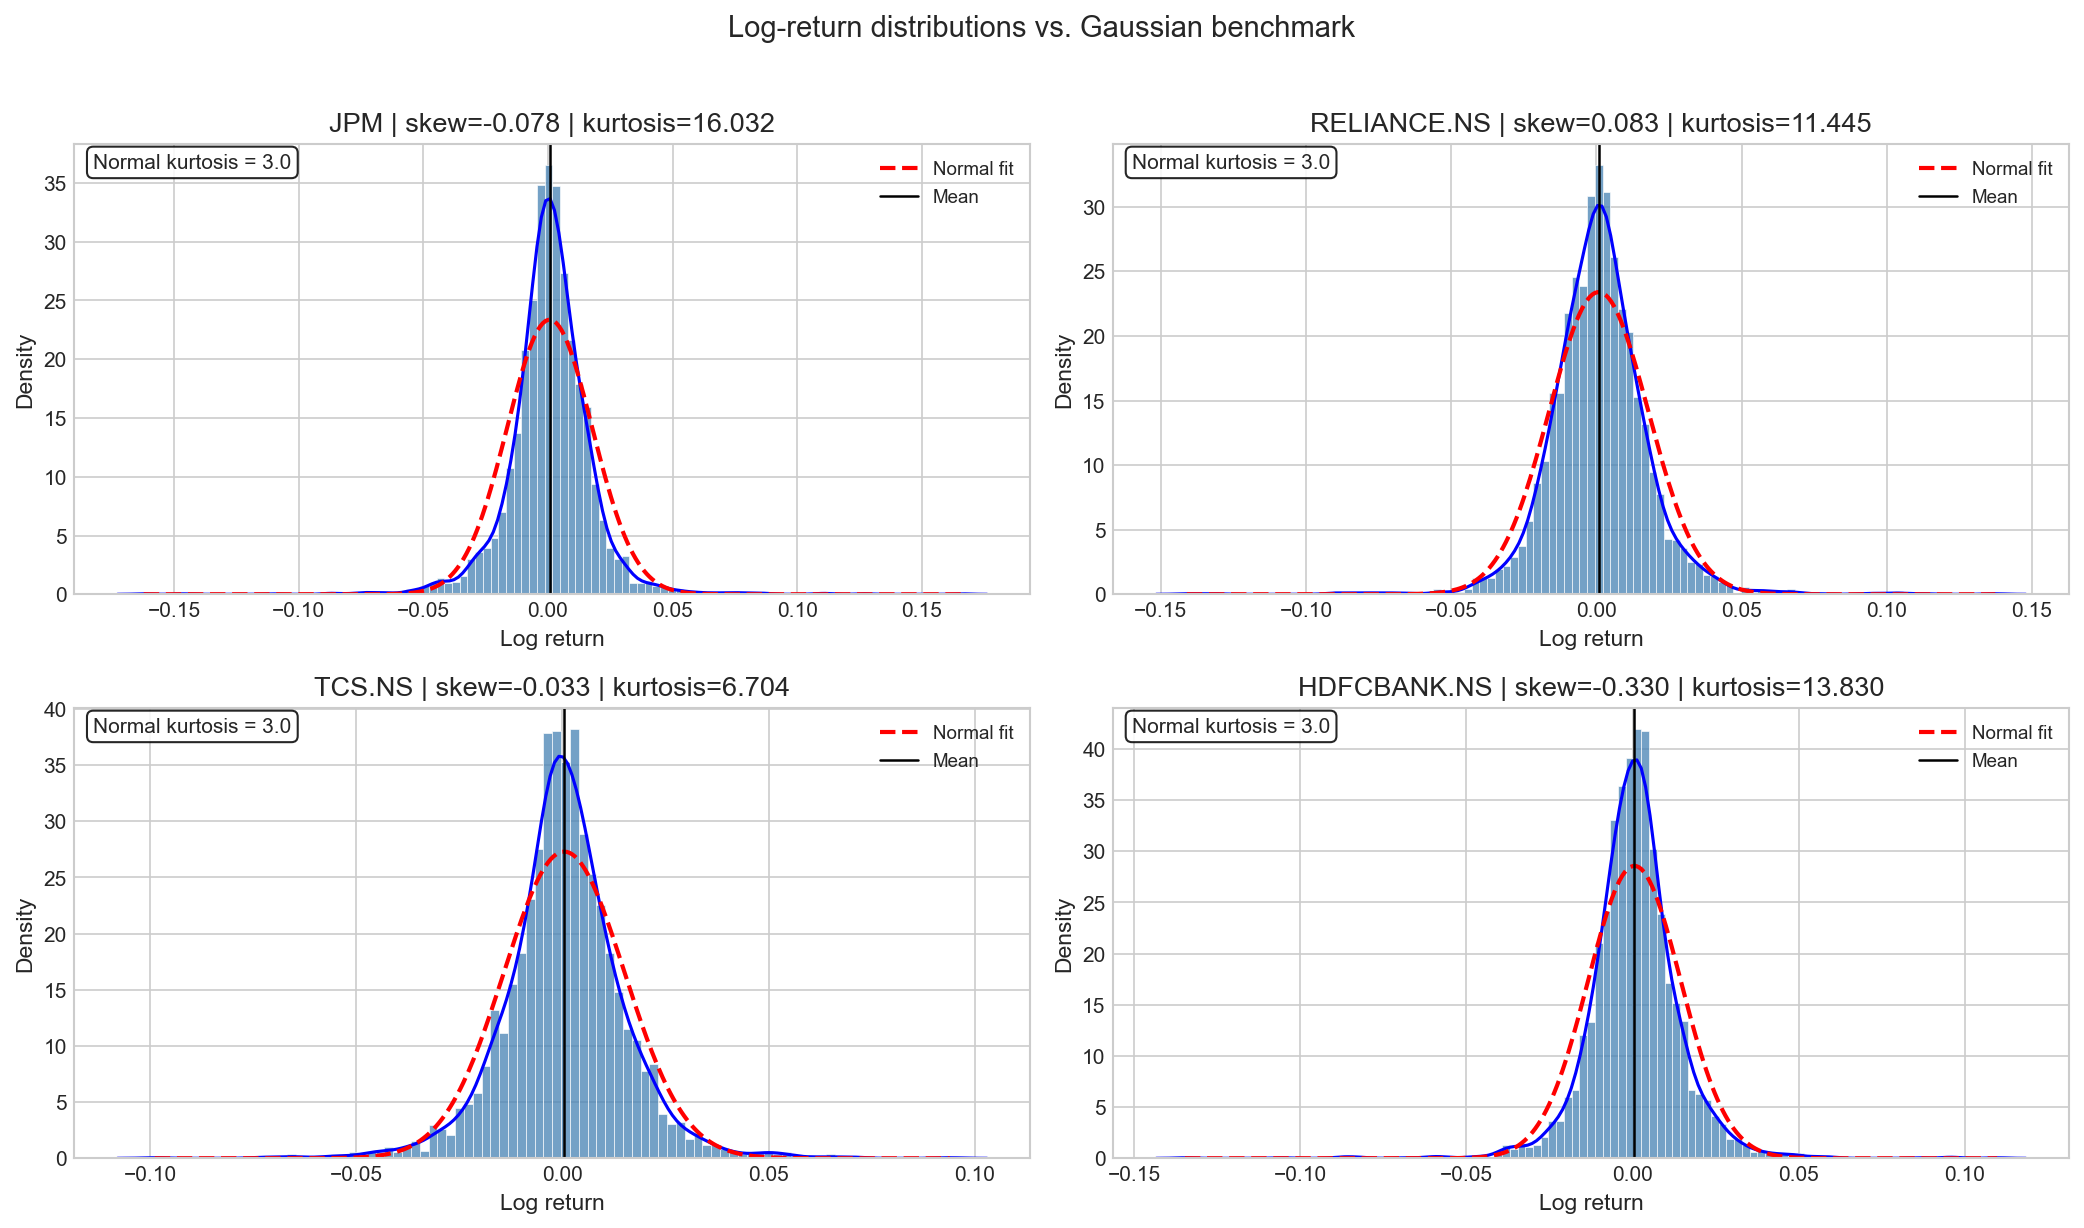
\includegraphics[width=\linewidth]{return_distributions.png}
\caption{Return distribution diagnostics (heavy tails and asymmetry) used to justify regime-aware modeling.}
\label{fig:return_dist}
\end{figure}

\begin{figure}[t]
\centering
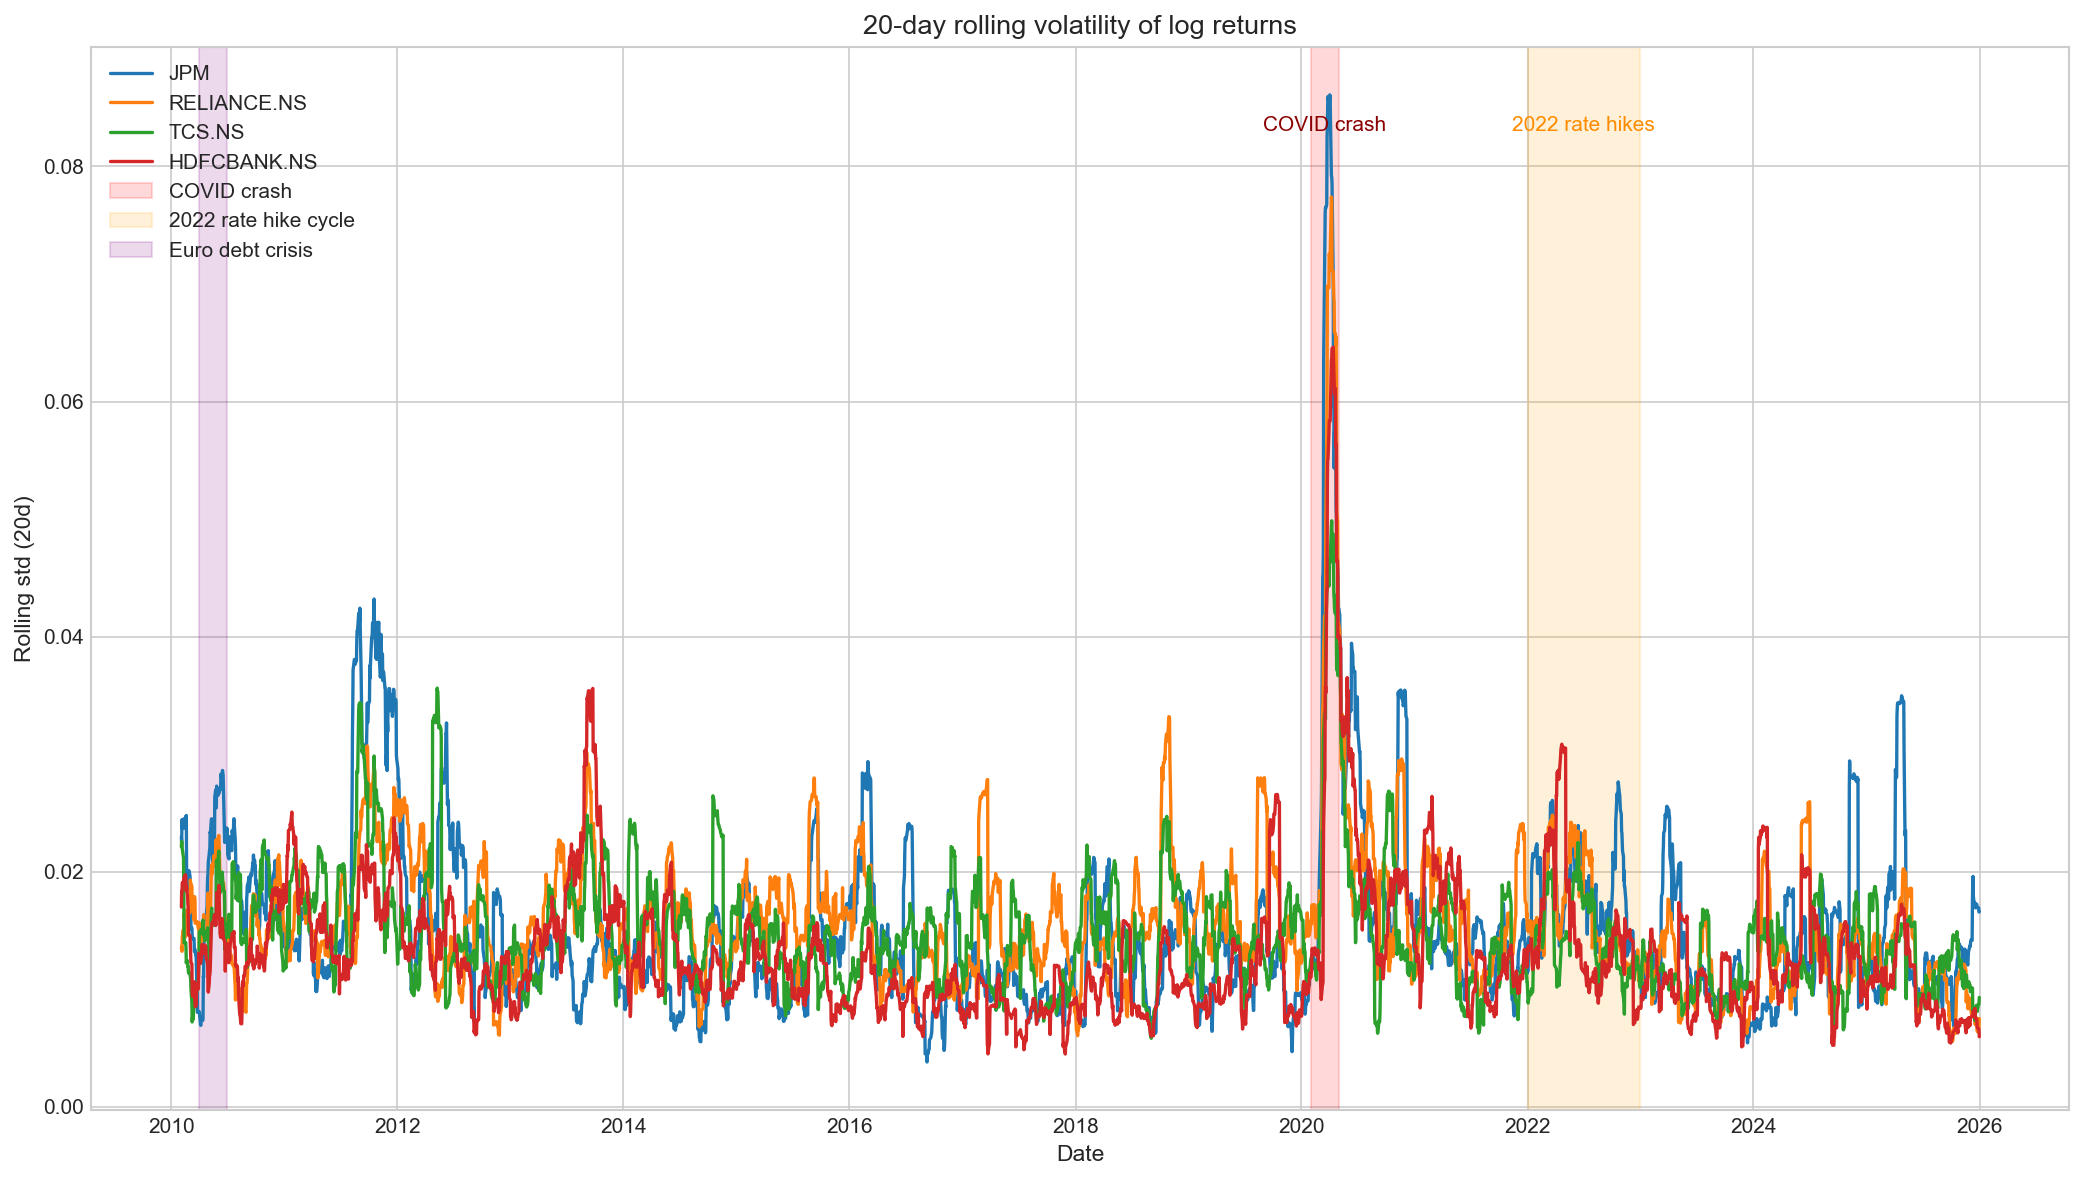
\includegraphics[width=\linewidth]{rolling_volatility.png}
\caption{20-day rolling volatility (actual EDA output), motivating explicit HMM state labeling.}
\label{fig:vol_regimes}
\end{figure}

\section{Preliminary Results (XGBoost Baseline)}
Table~\ref{tab:xgb_results} reports ticker-level baseline metrics from the confirmed regime-stratified run.

\begin{table}[t]
\centering
\caption{Regime-Stratified XGBoost: Main Results}
\label{tab:xgb_results}
\begin{tabular}{lcccc}
\toprule
Ticker & RMSE & MAE & DA (\%) & Sharpe \\
\midrule
JPM          & 0.0194 & 0.0127 & 52.13 & 0.53 \\
RELIANCE.NS  & 0.0180 & 0.0121 & 52.25 & 0.54 \\
TCS.NS       & 0.0151 & 0.0106 & 53.17 & 0.85 \\
HDFCBANK.NS  & 0.0165 & 0.0111 & 51.52 & 0.04 \\
EPIGRAL.NS   & 0.0243 & 0.0166 & 51.32 & -0.56 \\
\midrule
Average      & 0.0187 & 0.0126 & 52.08 & 0.28 \\
\bottomrule
\end{tabular}
\end{table}

Regime-stratified XGBoost achieves average DA of 52.08\%. TCS shows the strongest risk-adjusted result (Sharpe 0.85). HDFCBANK and EPIGRAL remain weak on Sharpe, consistent with noisy regime transitions and higher idiosyncratic effects in smaller names.

EPIGRAL.NS was included as a small-cap generalization test. Although DA is 51.32\%, the negative Sharpe (\(-0.56\)) indicates weak risk-adjusted behavior. This suggests OHLCV-only features are insufficient for small-cap settings and motivates multimodal signals (e.g., news sentiment and search-trend proxies) in Phase-2.

Table~\ref{tab:top5} summarizes the top-5 XGBoost feature-importance ranks for each ticker.

\begin{table}[!t]
\centering
\caption{Top-5 Features per Ticker (XGBoost Importance)}
\label{tab:top5}
\scriptsize
\setlength{\tabcolsep}{2pt}
\renewcommand{\arraystretch}{1.05}
\resizebox{\columnwidth}{!}{%
\begin{tabular}{lccccc}
\toprule
Ticker & R1 & R2 & R3 & R4 & R5 \\
\midrule
JPM         & Momentum\_60      & BB\_Lower      & BB\_Upper      & Rolling\_Corr\_Index & Momentum\_20 \\
RELIANCE.NS & Garman\_Klass\_Vol & MACD         & Return\_Lag\_2  & BB\_Position          & ROC\_10 \\
TCS.NS      & Momentum\_20      & BB\_Upper      & MACD\_Hist      & ROC\_10               & Momentum\_60 \\
HDFCBANK.NS & Momentum\_60      & Momentum\_20   & HMM\_Regime     & BB\_Lower             & MACD \\
EPIGRAL.NS  & HMM\_Regime       & ROC\_10        & Momentum\_20    & MACD\_Hist            & Rolling\_Corr\_Index \\
\bottomrule
\end{tabular}
}
\end{table}

HMM\_Regime appears in top-5 for HDFCBANK and EPIGRAL, providing direct evidence that regime labels carry predictive signal. Rolling\_Corr\_Index appears in top-5 for JPM and EPIGRAL, supporting the cross-asset context design.

\section{Conclusion}
Phase-1 is intentionally foundation-first: EDA, HMM regimes, engineered features, and a validated XGBoost baseline. This creates a strong technical base for later phases. The future architecture path (RAMT-style regime-gated multimodal transformer) remains a planned extension, not a claimed Phase-1 implementation.

\section*{Appendix: Phase 1 Rubric Mapping}
\begin{table}[t]
\centering
\caption{Phase-1 Rubric to Evidence Mapping}
\label{tab:rubric_map}
\scriptsize
\renewcommand{\arraystretch}{1.08}
\begin{tabular}{@{}>{\raggedright\arraybackslash}p{0.29\linewidth} >{\raggedright\arraybackslash}p{0.65\linewidth}@{}}
\toprule
Rubric Category & Evidence in This Submission \\
\midrule
Literature Review & Sec. II; ARIMA/GARCH limitations, SOTA comparison, explicit gap synthesis \cite{fanshawe2025,ying2026}. \\
Dataset Quality \& EDA & \path{eda/eda.ipynb}, figures in Fig.~\ref{fig:return_dist}, Fig.~\ref{fig:vol_regimes}. \\
Feature Engineering & \path{features/feature_engineering.py}; 36-column table, HMM regimes, cross-asset correlation. \\
Theoretical Rigor & HMM transition and emission equations in Sec. III-B. \\
Model Application & \path{models/baseline_xgboost.py}; walk-forward setup and Sec. IV results. \\
Code Quality / Reproducibility & Pipeline scripts in data/features/models, plus saved outputs in results. \\
Report Quality & IEEE format, equations, real figures, audited tables, and explicit phase scope. \\
\bottomrule
\end{tabular}
\end{table}

\balance
\begin{thebibliography}{99}

\bibitem{boxjenkins}
G.~E.~P. Box, G.~M. Jenkins, G.~C. Reinsel, and G.~M. Ljung, \emph{Time Series Analysis: Forecasting and Control}. Wiley, 2015.

\bibitem{engle1982}
R.~F. Engle, ``Autoregressive Conditional Heteroscedasticity with Estimates of the Variance of U.K. Inflation,'' \emph{Econometrica}, vol.~50, no.~4, pp. 987--1007, 1982.

\bibitem{bollerslev1986}
T.~Bollerslev, ``Generalized Autoregressive Conditional Heteroskedasticity,'' \emph{Journal of Econometrics}, vol.~31, no.~3, pp. 307--327, 1986.

\bibitem{rabiner1989}
L.~R. Rabiner, ``A Tutorial on Hidden Markov Models and Selected Applications in Speech Recognition,'' \emph{Proceedings of the IEEE}, vol.~77, no.~2, pp. 257--286, 1989.

\bibitem{xgboost2016}
T.~Chen and C.~Guestrin, ``XGBoost: A Scalable Tree Boosting System,'' in \emph{Proc. ACM SIGKDD}, 2016, pp. 785--794.

\bibitem{fanshawe2025}
J.~Fanshawe, R.~Masih, and A.~Cameron, ``Forecasting Equity Correlations with Hybrid Transformer Graph Neural Network,'' arXiv preprint, 2025.

\bibitem{ying2026}
Y.~Ying \emph{et al.}, ``Aligning News and Prices: A Cross-Modal LLM-Enhanced Transformer DRL Framework for Volatility-Adaptive Stock Trading,'' under review at ICLR, 2026.

\end{thebibliography}

\end{document}
